\section{Internal flow}
\frame{\tableofcontents[currentsection]}


\begin{frame}
    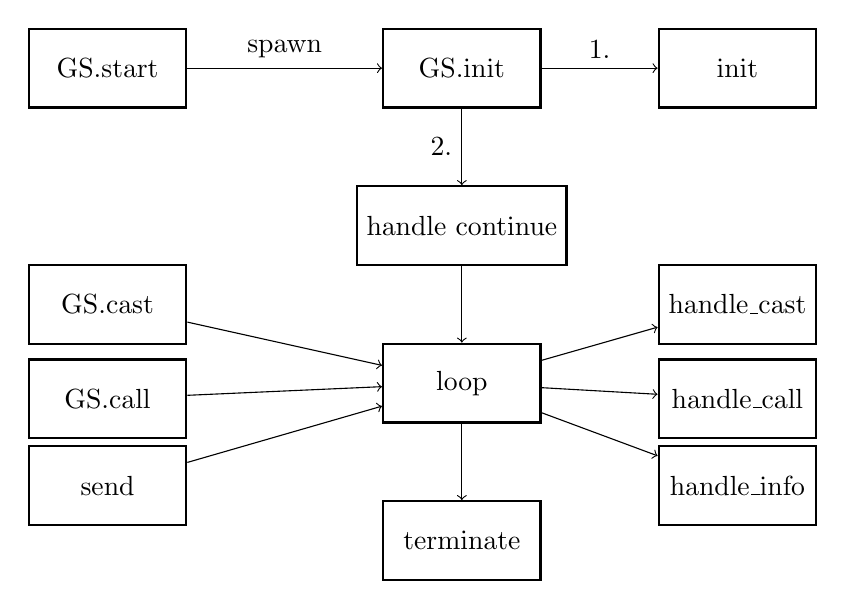
\begin{tikzpicture}
        % TODO kaderke
        \node (start) at (0,0) [draw,thick,minimum width=2cm,minimum height=1cm] {GS.start};
        \node (GSinit) at (4.5,0) [draw,thick,minimum width=2cm,minimum height=1cm] {GS.init};
        \node (init) at (8,0) [draw,thick,minimum width=2cm,minimum height=1cm] {init};

        \node (hco) at (4.5,-2) [draw,thick,minimum width=2cm,minimum height=1cm] {handle continue};
        \node (loop) at (4.5,-4) [draw,thick,minimum width=2cm,minimum height=1cm] {loop};

        \node (GScast) at (0,-3) [draw,thick,minimum width=2cm,minimum height=1cm] {GS.cast};
        \node (GScall) at (0,-4.2) [draw,thick,minimum width=2cm,minimum height=1cm] {GS.call};
        \node (send) at (0,-5.3) [draw,thick,minimum width=2cm,minimum height=1cm] {send};

        \node (hcast) at (8,-3) [draw,thick,minimum width=2cm,minimum height=1cm] {handle\_cast};
        \node (hcall) at (8,-4.2) [draw,thick,minimum width=2cm,minimum height=1cm] {handle\_call};
        \node (hinfo) at (8,-5.3) [draw,thick,minimum width=2cm,minimum height=1cm] {handle\_info};

        \node (term) at (4.5,-6) [draw,thick,minimum width=2cm,minimum height=1cm] {terminate};

        \draw[->] (start) to node[anchor=south][black]{spawn} (GSinit);
        \draw[->] (GSinit) to node[anchor=south][black]{1.} (init);

        \draw[->] (GSinit.south) to node[anchor=east][black]{2.} (hco.north);
        \draw[->] (hco.south) -- (loop.north);
        
        \draw[->] (GScast) -- (loop);
        \draw[->] (GScall) -- (loop);
        \draw[->] (send) -- (loop);
        
        \draw[->] (loop) -- (hcast);
        \draw[->] (loop) -- (hcall);
        \draw[->] (loop) -- (hinfo);

        \draw[->] (loop) -- (term);
    \end{tikzpicture}
    \vfill
    \tiny \textit{Note that there are 2 parts. The API (left column) and the server callbacks (middle/right columns)}
\end{frame}
% Note: GS.init is actually proc_lib:init_ack/1,2. 
%  see https://marcelog.github.io/articles/erlang_special_processes_tutorial_handling_system_messages.html
%   How it works section